\documentclass[
  11pt, % The default document font size, options: 10pt, 11pt, 12pt
  codirector, % Uncomment to add a codirector to the title page
]{charter}
\usepackage{enumitem}
\usepackage{pdflscape}
\usepackage{tikz}
%\usetikzlibrary{shapes,arrows}
%\usepackage{tikz}
\usetikzlibrary{positioning, arrows.meta, backgrounds, fit}
\usepackage{fontawesome5}
\usepackage{tikz,tkz-tab}
\usepackage{booktabs} % Para tablas más elegantes
\usetikzlibrary{positioning, arrows.meta, backgrounds, fit}

\usetikzlibrary{matrix,arrows, positioning,shadows,shadings,backgrounds, calc, shapes, tikzmark}

\usepackage{fmtcount}
\usepackage{xurl}



% Completar los siguintes Campos
\materia{Circuitos Logicos Programables}
\bimestre{cuarto bimestre}
\docentes{Nicolás Alvarez}
\titulo{ALU Sparc v8}
\posgrado{Carrera de Especialización en Sistemas Embebidos}
\autor{Ing. Iriarte Fernandez, Nicolás Ezequiel
  (NicolasIriarte95@gmail.com)}
\director{}
\pertenenciaDirector{}
\codirector{}
\pertenenciaCoDirector{}
\fechaINICIO{11 de Abril de 2024}

\begin{document}

\maketitle
\tableofcontents

\newpage

\section*{Registros de cambios}
\label{sec:registro}


\begin{table}[ht]
	\label{tab:registro}
	\centering
	\begin{tabularx}{\linewidth}{@{}|c|X|c|@{}}
		\hline
		\rowcolor[HTML]{C0C0C0}
		Revisión & \multicolumn{1}{c|}{\cellcolor[HTML]{C0C0C0}Detalles de los cambios realizados} & Fecha      \\ \hline
		0      & Creación del documento.                                 &\fechaInicioName \\ \hline

    		1      & Se aplican cambios sugeridos por Salamandri Santiago. & 20 de noviembre de 2023 \\ \hline


    \hline

	\end{tabularx}
	\label{sec:cierre}
\end{table}

%% \pagebreak


%%%%%%%%%%%%%%%%%%%%%%%%%%%%%%%%%%%%%%%%%%%%%%%%%%
\section*{Documentos anexos}
\label{sec:documentos_anexos}

\begin{table}[h!]
	\centering
	\begin{tabular}{ | m{1.5cm} | m{3cm} | m{10.5cm} | }
		\hline
		\rowcolor{gray!50} % Coloring the first row
		\textbf{Ref.} & \textbf{Nombre} & \textbf{Descripción} \\ \hline
    AD.01 & SPARC\-V8\-AM & Especificación de requerimientos de software. \\ \hline
	\end{tabular}
  \caption{Documentos anexos.}
  \label{tab:referencias}

\end{table}
%%%%%%%%%%%%%%%%%%%%%%%%%%%%%%%%%%%%%%%%%%%%%%%%%%

\section*{Glosario}
\label{sec:glossary}

\begin{table}[h!]
	\centering
	\begin{tabular}{ | m{4.5cm} | m{10.5cm} | }
		\hline
		\rowcolor{gray!50} % Coloring the first row
		\textbf{Acronimo} & \textbf{Definición} \\ \hline
    ALU  & Unidad Aritnética Lógica. \\ \hline
    CLP  & Circuitos Lógicos Programables. \\ \hline
    ICC & Integer Condition Code. \\ \hline
    SPARC  & Scalable Processor Architecture. \\ \hline
	\end{tabular}
  \caption{Glosario.}
  \label{tab:glossary}

\end{table}
%%%%%%%%%%%%%%%%%%%%%%%%%%%%%%%%%%%%%%%%%%%%%%%%%%
\pagebreak


\section{Introducción}
\label{sec:org60390fa}

En el presente documento se detallarán los aspectos relacionados con el desarrollo e implementación del trabajo final de la matería ``Circuitos Lógicos Programables (CLP)''. El cual consiste en una ALU de la arquitectura Sparc V8 tal como se describe en \textbf{AD.01}.

\section{Desarrollo, alcance y limitaciones}
\label{sec:orgaf51da6}

El desarrollo del trabajo final se realizaró en el lenguaje de descripción de
hardware VHDL. Y se implementaó una ALU de 32 bits que soportará las operaciones
aritméticas y lógicas básicas. Durante el planeamiento y desarrollo se intentó
representar la arquitectura Sparc V8 de forma fiel, sin embargo, para limitar el
alcance del trabajo final se decidieron hacer las siguientes simplificaciones:

\begin{itemize}
\item El componente no tiene clock asociado, por lo que la actualización de
  cualquier de sus entradas genera una salida.
\item Se implementaron unicamente las siguientes instrucciones, respetando el
  formato de la trama tal como en el manual de arquitectura
  (\textbf{AD.01 Pag. 43}). Las instrucciones implementadas son:
  \begin{itemize}
  \item \textbf{ADDcc (Opcode: 010000)}: Adición con actualización de ICC.
  \item \textbf{SUBcc (Opcode: 010100)}: Resta con actualización de ICC.
  \item \textbf{UMULcc (Opcode: 011010)}: Multiplicación sin signo con actualización de ICC.
  \item \textbf{SMULcc (Opcode: 011011)}: Multiplicación con signo con actualización de ICC.
  \end{itemize}
\item Para simplificación, el mecanismo de ventanas descrito en el manual de
  arquitectura (\textbf{AD.01 Pag. 27}) no fue implementado. Y para recuperar
  los valores de algunos registros requeridos, se pasaron directamente como
  \textbf{señales} al componente.
\end{itemize}

A partir de estas simplificaciones, el componente ``ALU'' que se implementó
tiene la siguiente estructura interna:

\newpage

\begin{figure}[htpb]
  \centering
  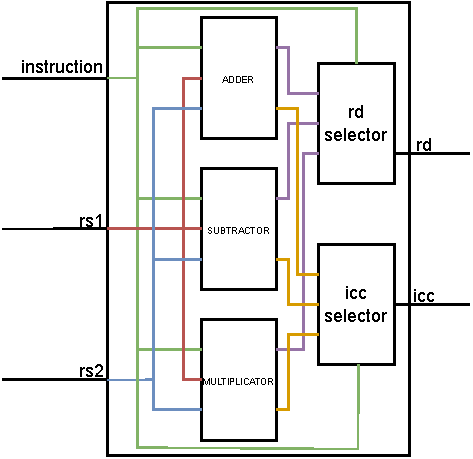
\includegraphics[width=.5\textwidth]{./Figuras/Components.pdf}
  \caption{Diagrama de componentes.}
  \label{fig:Components}
\end{figure}

\vspace{25px}

Tal como se observa en la Figura \ref{fig:Components}, el componente ``ALU''
tiene tres entradas:

\begin{enumerate}
\item \textbf{instruction}: Señal de 32 bits que contiene la instrucción a
  ejecutar. La instrucción se decodifica y se extraen los campos necesarios para
  la ejecución de la operación. Para mayor información en el formato de la
  instrucción ver \textbf{AD.01}.
\item \textbf{rs1}: Señal de 32 bits que contiene el valor del registro fuente
  \textbf{RS1}.
\item \textbf{rs2}: Señal de 32 bits que contiene el valor del registro fuente
  \textbf{RS2}.
\end{enumerate}

Y dos salidas:

\begin{enumerate}
\item \textbf{rd}: Señal de 32 bits que contiene resultado de la operación a ejecutar.
\item \textbf{icc}: Señal de 4 bits que contiene el valor del Integer Condition
  Code (ICC) actualizado. Para mayor información en el formato del ICC ver
  \textbf{AD.01 Pag. 28}.
\end{enumerate}

Como filosofía de diseño, se optó por tenér un sub-componente para cada una de
las instrucciones soportadas por la ALU, permitiendo de esta manera generar
código VHDL más segmentado y limpio.

Dicho diseño tiene la desventaja de que todas las entradas y salidas de cada
sub-componente están conectadas entre sí, y a demás, se debe agregar un selector
por cada uno de las salidas esperadas.

El selector se encargará de interpretár la instrucción recibida, extraerá su
Opcode y dependiendo de este último, seleccionará que sub-componente
redireccionar como salida del mismo.

\section{Simulaciones}
\label{sec:org0000000}

Durante el desarrollo del presente trabajo, se realizaron multiples simulaciones de distintas entradas e instrucciones para verificar el correcto funcionamiento de los componentes implementados. Dichas entradas buscaron verificar distintos aspectos, tales como correcto funcionamiento de los ICC, busqueda de overflows, correcto calculo e interpretación de valores negativos. A continuación se deja un grafico generado a partir de la simulación del test-bench generado:

%% \newpage

\begin{figure}[htpb]
  \centering
  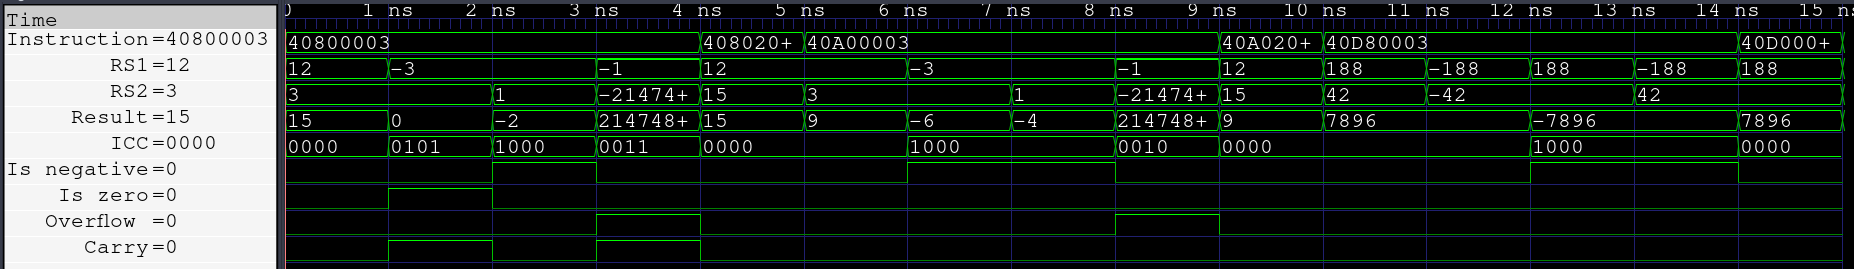
\includegraphics[width=1\textwidth]{./Figuras/gtkwave.png}
  \caption{Simulación en Gtk-Wave.}
  \label{fig:gtkwave}
\end{figure}

\vspace{25px}

\section{Resumen del proyecto}
\label{sec:org0000001}

Tras su desarrollo e implementación, se pudo sintetizar las operaciones deseadas. Generando de esta manera el siguiente resumen por parte de Vivado:

\begin{figure}[htpb]
  \centering
  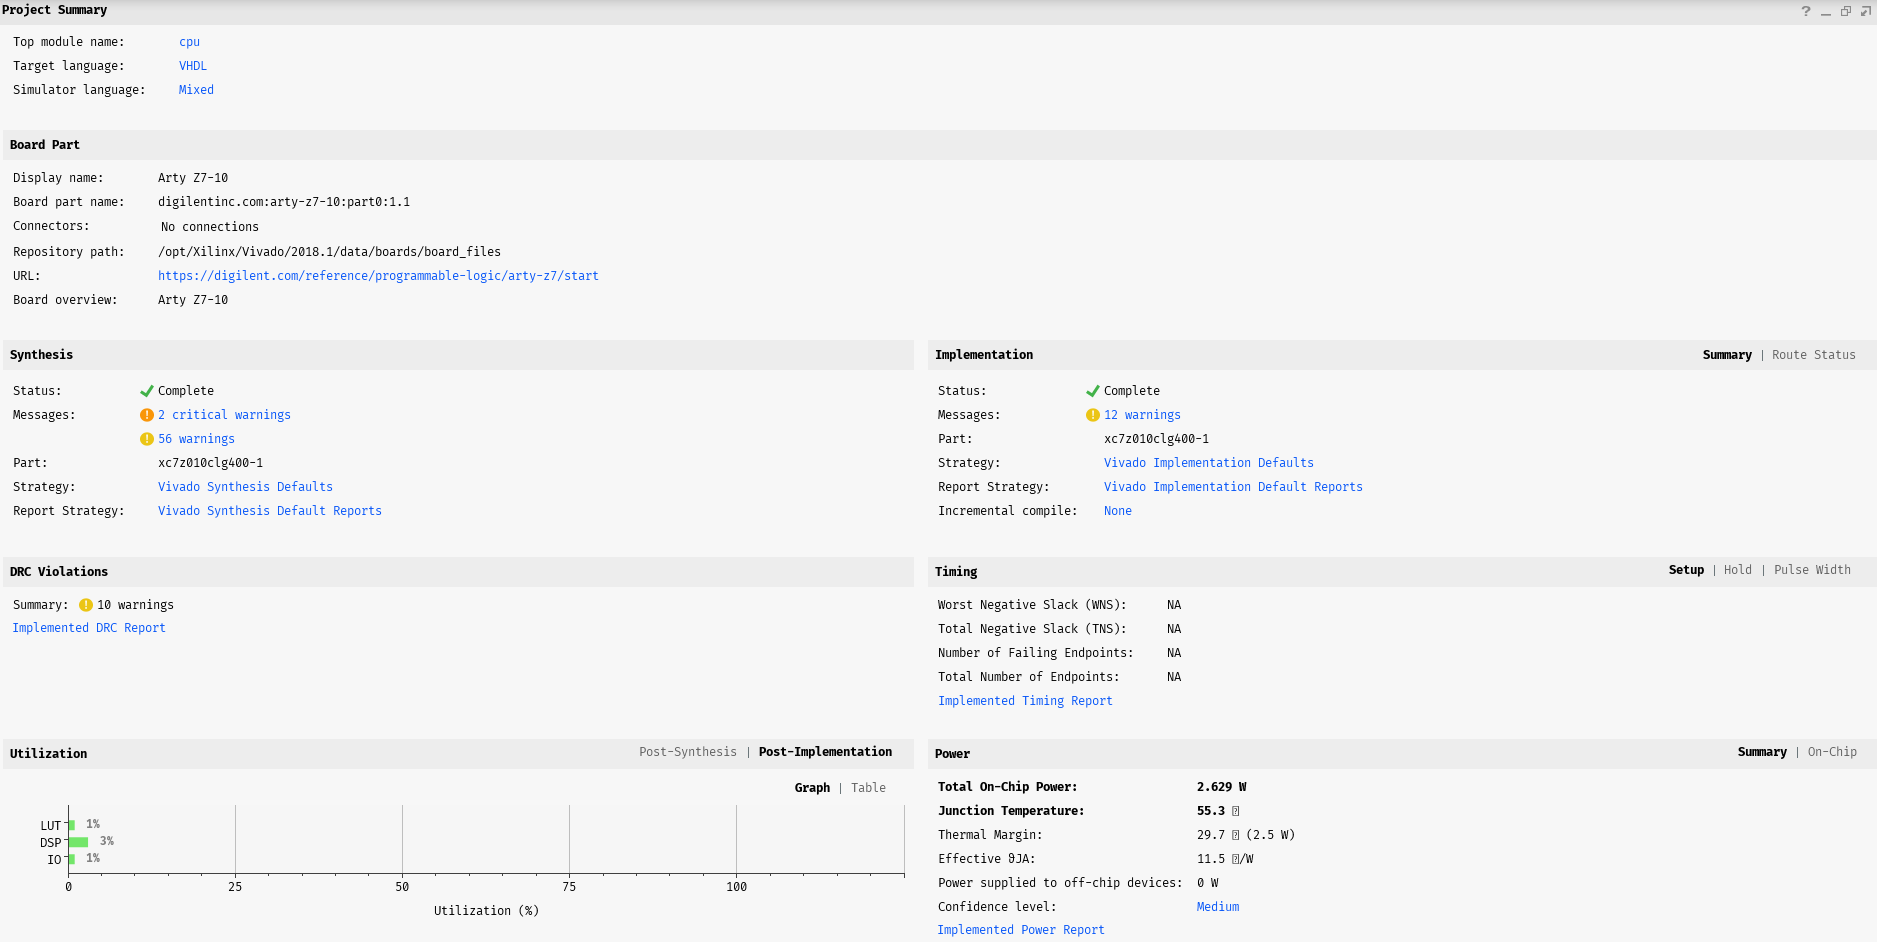
\includegraphics[width=1\textwidth]{./Figuras/project-summary.png}
  \caption{Resumen del proyecto por parte de la herramienta Vivado.}
  \label{fig:project-summary}
\end{figure}

\vspace{25px}

\newpage

\begin{figure}[htpb]
  \centering
  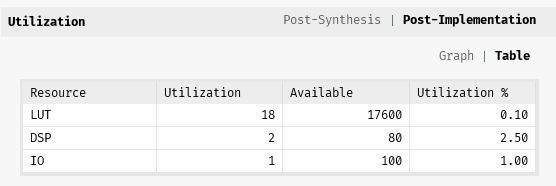
\includegraphics[width=.5\textwidth]{./Figuras/utilization-table.png}
  \caption{Tabla de utilización de recursos.}
  \label{fig:utilization-table}
\end{figure}

\vspace{25px}

\section{Anexos}

\subsection{Ejemplo instrucción ADDcc}
Dicha trama se explica en mayor detalle en el documento \textbf{AD.01} en la página 106 y 170. Tenér en cuenta que se hicieron algunas simplificaciones, tal como solo implementar las variaciones en donde el ICC es actualizado.

\begin{figure}[htpb]
  \centering
  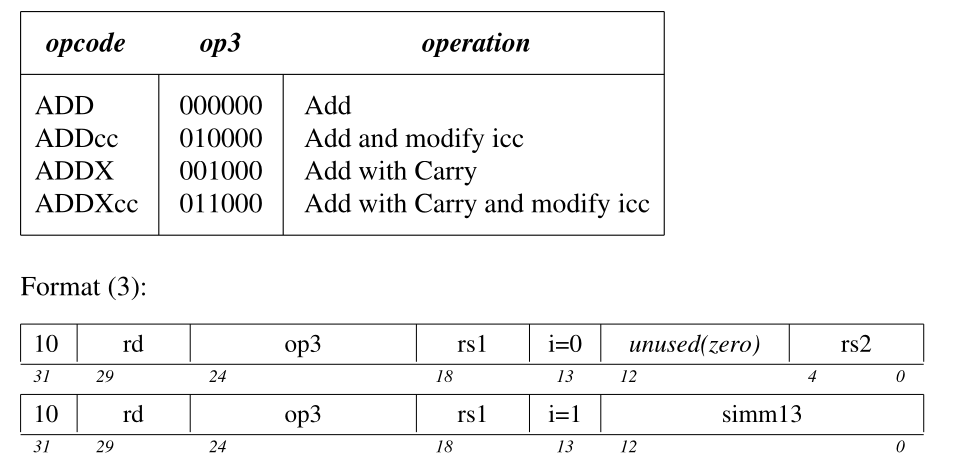
\includegraphics[width=.8\textwidth]{./Figuras/addcc-format.png}
  \caption{Formato de trama en instrucción ``ADDcc''.}
  \label{fig:addcc-format}
\end{figure}

\vspace{25px}
\newpage

\begin{figure}[htpb]
  \centering
  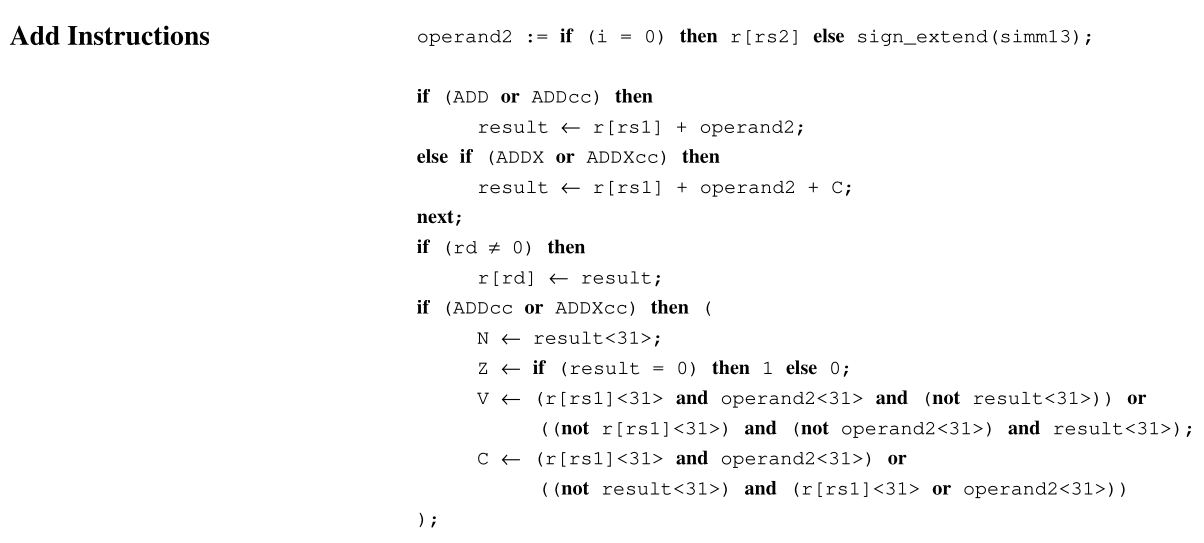
\includegraphics[width=1\textwidth]{./Figuras/addcc-logic.png}
  \caption{Comportamiento de la instrucción ``ADDcc''.}
  \label{fig:addcc-logic}
\end{figure}

\vspace{25px}


\end{document}
